\documentclass[aspectratio=169, 11pt]{beamer}

% --- Packages & Setup ---
\usepackage[utf8]{inputenc}
\usepackage[T1]{fontenc}
\usepackage{xcolor}
\usepackage{booktabs}
\usepackage{array}
\usepackage{graphicx}
\usepackage{tikz}
\usetikzlibrary{calc,arrows.meta,positioning,shapes.geometric}

\graphicspath{{../}{./}}

% Try loading Open Sans; fallback if missing
\IfFileExists{opensans.sty}{\usepackage[default,scale=0.95]{opensans}}{}

% --- Branding Colors ---
\definecolor{amritaMaroon}{HTML}{A4123F}
\definecolor{maroonSoft}{HTML}{F6E3E9}
\definecolor{inkGray}{HTML}{3A3A3A}
\definecolor{goldAccent}{HTML}{C79A3A}

% --- Theme Setup ---
\usetheme{Madrid}
\usecolortheme[named=amritaMaroon]{structure}
\setbeamertemplate{navigation symbols}{}
\setbeamertemplate{footline}[frame number]

% node styles reused across diagrams
\tikzset{
  lbl/.style={circle, draw=amritaMaroon, thick, fill=maroonSoft, minimum size=1.05cm, font=\scriptsize, align=center},
  lblcenter/.style={circle, draw=amritaMaroon, very thick, fill=amritaMaroon, text=white, minimum size=1.15cm, font=\bfseries\scriptsize, align=center},
  edg/.style={-, thick, draw=inkGray},
  edgfaint/.style={-, draw=inkGray!35},
  edghi/.style={-, ultra thick, draw=amritaMaroon},
  stepbox/.style={rectangle, draw=amritaMaroon, thick, fill=maroonSoft, rounded corners=2pt, minimum width=3.4cm, minimum height=0.75cm, font=\footnotesize, align=center}
}

% small icon-in-circle helpers for the Applications slide
\newcommand{\iconGraph}{%

\begin{tikzpicture}
\node[circle, fill=amritaMaroon, minimum size=0.9cm] (bg) {};
\node[circle, fill=white, minimum size=0.11cm, inner sep=0pt] (a) at ($(bg.center)+(-0.18,0.15)$) {};
\node[circle, fill=white, minimum size=0.11cm, inner sep=0pt] (b) at ($(bg.center)+(0.18,0.15)$) {};
\node[circle, fill=white, minimum size=0.11cm, inner sep=0pt] (c) at ($(bg.center)+(0,-0.2)$) {};
\draw[white, thin] (a) -- (b) -- (c) -- (a);
\end{tikzpicture}}

\newcommand{\iconMagnify}{%

\begin{tikzpicture}
\node[circle, fill=amritaMaroon, minimum size=0.9cm] (bg) {};
\draw[white, thick] ($(bg.center)+(-0.05,0.1)$) circle (0.17cm);
\draw[white, thick, line cap=round] ($(bg.center)+(0.07,-0.02)$) -- ($(bg.center)+(0.27,-0.24)$);
\end{tikzpicture}}

\newcommand{\iconDNA}{%

\begin{tikzpicture}
\node[circle, fill=amritaMaroon, minimum size=0.9cm] (bg) {};
\draw[white, thick] ($(bg.center)+(-0.2,0.28)$) .. controls ($(bg.center)+(0.2,0.12)$) and ($(bg.center)+(-0.2,-0.12)$) .. ($(bg.center)+(0.2,-0.28)$);
\draw[white, thick] ($(bg.center)+(0.2,0.28)$) .. controls ($(bg.center)+(-0.2,0.12)$) and ($(bg.center)+(0.2,-0.12)$) .. ($(bg.center)+(-0.2,-0.28)$);
\end{tikzpicture}}

\newcommand{\iconLeaf}{%

\begin{tikzpicture}
\node[circle, fill=amritaMaroon, minimum size=0.9cm] (bg) {};
\draw[white, thick] ($(bg.center)+(0,-0.3)$) -- ($(bg.center)+(0,0.05)$);
\filldraw[white] ($(bg.center)+(0.02,0.2)$) ellipse[x radius=0.22cm, y radius=0.13cm, rotate=40];
\draw[amritaMaroon, thin] ($(bg.center)+(-0.13,0.11)$) -- ($(bg.center)+(0.17,0.29)$);
\end{tikzpicture}}

\begin{document}

\begin{frame}
    \titlepage
    \begin{center}
        \textbf{Evaluating Graph Representations using Weisfeiler-Lehman Graph Kernels} \\
        \vspace{0.2cm}
        Plant Trait Analysis using OLID
    \end{center}
\end{frame}

% ============================================================
% FRAME: What is the WL Graph Kernel?
% ============================================================
\begin{frame}{What is the WL Graph Kernel?}
    \framesubtitle{Weisfeiler--Lehman (WL) Graph Kernel}
    \begin{columns}[c]
        \column{0.52\textwidth}
        \textbf{Main idea}
        \vspace{0.15cm}

        The WL graph kernel compares graphs by \textbf{iteratively capturing the
        labels of each node and its neighborhood}.

        \vspace{0.3cm}
        \begin{itemize}
            \item Every node starts with a simple label.
            \item Labels are repeatedly updated using neighboring labels.
            \item The resulting label patterns are turned into a
            feature vector used to measure \textbf{similarity between graphs}.
        \end{itemize}

        \column{0.44\textwidth}
        \centering
        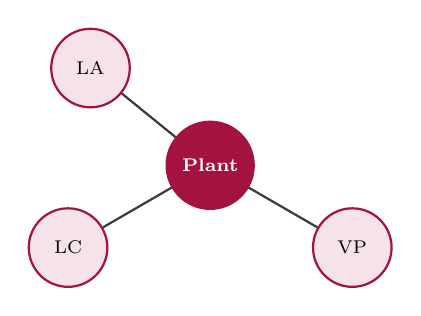
\begin{tikzpicture}[scale=0.95, every node/.style={transform shape}]
            \node[lblcenter] (p) at (0,0) {Plant};
            \node[lbl] (la) at (-1.6,1.3) {LA};
            \node[lbl] (lc) at (-1.9,-1.1) {LC};
            \node[lbl] (vp) at (1.9,-1.1) {VP};
            \draw[edg] (p) -- (la);
            \draw[edg] (p) -- (lc);
            \draw[edg] (p) -- (vp);
        \end{tikzpicture}

        \vspace{0.1cm}
        {\scriptsize\itshape A node's label evolves by absorbing
        information from its neighbors.}
    \end{columns}
\end{frame}

% ============================================================
% FRAME: How Does WL Work? (1/2) -- labels + aggregation
% ============================================================
\begin{frame}{How Does WL Work?}
    \begin{columns}[t]
        \column{0.48\textwidth}
        \textbf{1. Start with node labels}

        \vspace{0.1cm}
        {\footnotesize Each graph node has an initial label:}
        \begin{itemize}\footnotesize
            \item Plant $\rightarrow$ \texttt{plant}
            \item LA $\rightarrow$ \texttt{LA\_low}
            \item LC $\rightarrow$ \texttt{LC\_high}
            \item VP $\rightarrow$ \texttt{VP\_medium}
        \end{itemize}

        \vspace{0.25cm}
        \textbf{2. Iteratively aggregate neighborhood information}

        \vspace{0.1cm}
        {\footnotesize For each node:}

        \begin{center}
        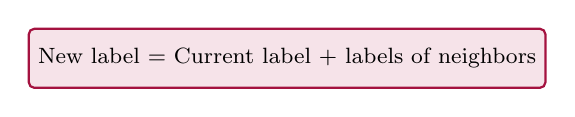
\begin{tikzpicture}
            \node[stepbox] {New label = Current label + labels of neighbors};
        \end{tikzpicture}
        \end{center}

        \column{0.48\textwidth}
        \centering
        {\footnotesize\textbf{Before}}\\[0.15cm]
        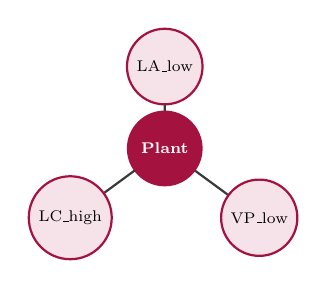
\begin{tikzpicture}[scale=0.8, every node/.style={transform shape}]
            \node[lbl] (la) at (0,1.3) {LA\_low};
            \node[lblcenter] (p) at (0,0) {Plant};
            \node[lbl] (lc) at (-1.5,-1.1) {LC\_high};
            \node[lbl] (vp) at (1.5,-1.1) {VP\_low};
            \draw[edg] (p) -- (la);
            \draw[edg] (p) -- (lc);
            \draw[edg] (p) -- (vp);
        \end{tikzpicture}

        \vspace{0.35cm}
        {\footnotesize\textbf{After WL iteration}}\\[0.1cm]
        {\scriptsize
        \begin{tabular}{@{}l@{}}
            Plant $\rightarrow$ plant \textbar\ LA\_low \textbar\ LC\_high \textbar\ VP\_low \\
            LA \quad\ $\rightarrow$ LA\_low \textbar\ plant \\
            LC \quad\ $\rightarrow$ LC\_high \textbar\ plant \\
            VP \quad\ $\rightarrow$ VP\_low \textbar\ plant \\
        \end{tabular}}
    \end{columns}
\end{frame}

% ============================================================
% FRAME: How Does WL Work? (2/2) -- feature vector + key point
% ============================================================
\begin{frame}{How Does WL Work? \textnormal{\footnotesize(contd.)}}
    \textbf{3. Build a feature representation}

    \vspace{0.05cm}
    {\footnotesize The labels generated at each WL iteration are counted to form
    a WL feature vector.}

    \vspace{0.08cm}
    \begin{center}
    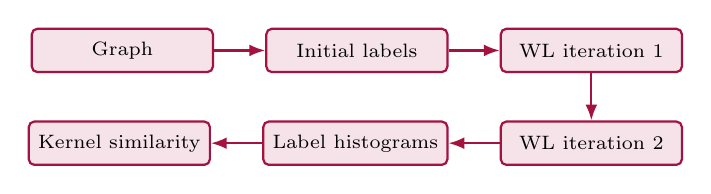
\begin{tikzpicture}[every node/.style={transform shape}]
        \tikzset{stepboxsm/.style={rectangle, draw=amritaMaroon, thick, fill=maroonSoft,
              rounded corners=2pt, minimum width=2.3cm, minimum height=0.55cm, font=\scriptsize, align=center}}
        \node[stepboxsm] (g)  {Graph};
        \node[stepboxsm, right=0.65cm of g] (il) {Initial labels};
        \node[stepboxsm, right=0.65cm of il] (i1) {WL iteration 1};
        \node[stepboxsm, below=0.6cm of i1] (i2) {WL iteration 2};
        \node[stepboxsm, left=0.65cm of i2] (lh) {Label histograms};
        \node[stepboxsm, left=0.65cm of lh] (ks) {Kernel similarity};
        \draw[-{Latex[length=2mm]}, thick, draw=amritaMaroon] (g) -- (il);
        \draw[-{Latex[length=2mm]}, thick, draw=amritaMaroon] (il) -- (i1);
        \draw[-{Latex[length=2mm]}, thick, draw=amritaMaroon] (i1) -- (i2);
        \draw[-{Latex[length=2mm]}, thick, draw=amritaMaroon] (i2) -- (lh);
        \draw[-{Latex[length=2mm]}, thick, draw=amritaMaroon] (lh) -- (ks);
    \end{tikzpicture}
    \end{center}

    \vspace{0.1cm}
    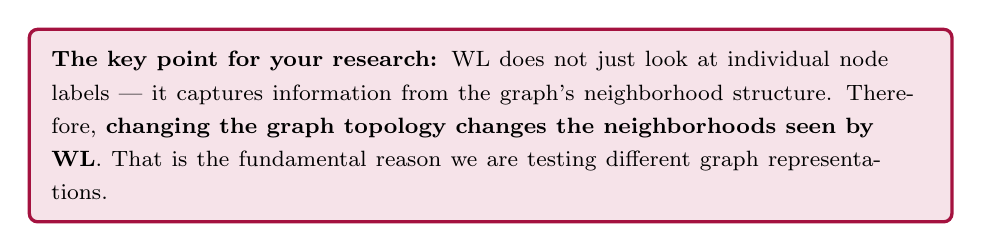
\begin{tikzpicture}
        \node[rectangle, draw=amritaMaroon, very thick, fill=maroonSoft,
              rounded corners=3pt, inner sep=8pt, text width=0.92\textwidth] {
            \footnotesize
            \textbf{The key point for your research:} WL does not just look at
            individual node labels --- it captures information from the graph's
            neighborhood structure. Therefore, \textbf{changing the graph
            topology changes the neighborhoods seen by WL}. That is the
            fundamental reason we are testing different graph representations.
        };
    \end{tikzpicture}
\end{frame}

% ============================================================
% FRAME: WL Algorithm -- Mathematical Formulation
% ============================================================
\begin{frame}{WL Algorithm: Mathematical Formulation}
    \framesubtitle{The formal update rule behind the visual picture}

    \begin{center}
        \Large
        $$ l_i(v) = f\left(l_{i-1}(v),\ \{\!\{\, l_{i-1}(u) : u \in N(v) \,\}\!\}\right) $$
    \end{center}

    \vspace{0.2cm}
    \begin{itemize}
        \item $l_i(v)$ -- the label of node $v$ after iteration $i$.
        \item $l_{i-1}(v)$ -- the node's own label from the previous iteration.
        \item $N(v)$ -- the set of neighbors of $v$.
        \item $\{\!\{\, l_{i-1}(u) : u \in N(v) \,\}\!\}$ -- the \textbf{multiset}
        of neighbor labels (order doesn't matter, repeats are kept).
        \item $f$ -- a hashing/compression function that combines a node's own
        label with its neighbors' labels into a new, compact label.
    \end{itemize}

    \vspace{0.15cm}
    {\footnotesize\itshape This is exactly the "current label + neighbor
    labels" update shown on the previous slide, written formally.}
\end{frame}

% ============================================================
% FRAME: Why Graph Representation Matters
% ============================================================
\begin{frame}{Why Graph Representation Matters}
    \framesubtitle{Same six traits, two different topologies}

    \begin{columns}[t]
        \column{0.48\textwidth}
        \centering
        {\footnotesize\textbf{Star graph}}\\[0.1cm]
        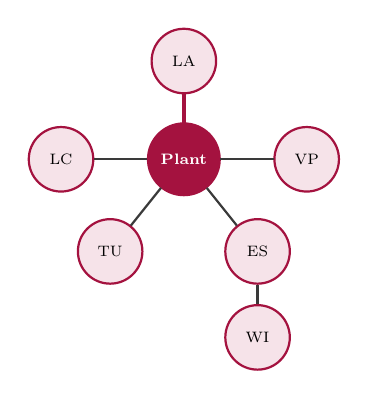
\begin{tikzpicture}[scale=0.78, every node/.style={transform shape}]
            \node[lbl] (la) at (0,1.6)   {LA};
            \node[lblcenter] (p) at (0,0) {Plant};
            \node[lbl] (lc) at (-2.0,0)  {LC};
            \node[lbl] (vp) at (2.0,0)   {VP};
            \node[lbl] (tu) at (-1.2,-1.5) {TU};
            \node[lbl] (es) at (1.2,-1.5)  {ES};
            \node[lbl] (wi) at (1.2,-2.9)  {WI};
            \draw[edghi] (p) -- (la);
            \draw[edg] (p) -- (lc);
            \draw[edg] (p) -- (vp);
            \draw[edg] (p) -- (tu);
            \draw[edg] (p) -- (es);
            \draw[edg] (es) -- (wi);
        \end{tikzpicture}

        \vspace{0.15cm}
        {\footnotesize LA sees only: \; LA $\rightarrow$ Plant}

        \column{0.48\textwidth}
        \centering
        {\footnotesize\textbf{Fully connected graph}}\\[0.1cm]
        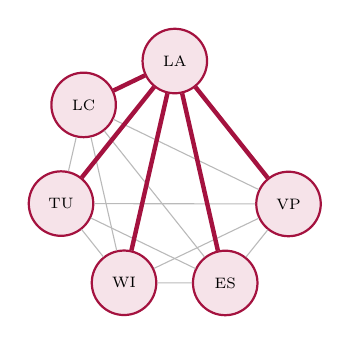
\begin{tikzpicture}[scale=0.78, every node/.style={transform shape}]
            \foreach \name/\ang in {LA/90, LC/141.4, TU/192.8, WI/244.2, ES/295.6, VP/347}
                \node[lbl] (\name) at (\ang:1.9) {\name};
            \foreach \a/\b in {LA/LC, LA/TU, LA/WI, LA/ES, LA/VP,
                               LC/TU, LC/WI, LC/ES, LC/VP,
                               TU/WI, TU/ES, TU/VP,
                               WI/ES, WI/VP, ES/VP}
                \draw[edgfaint] (\a) -- (\b);
            \foreach \b in {LC,TU,WI,ES,VP}
                \draw[edghi] (LA) -- (\b);
        \end{tikzpicture}

        \vspace{0.15cm}
        {\footnotesize LA sees all of: \; LA $\rightarrow$ LC, VP, TU, ES, WI}
    \end{columns}

    \vspace{0.3cm}
    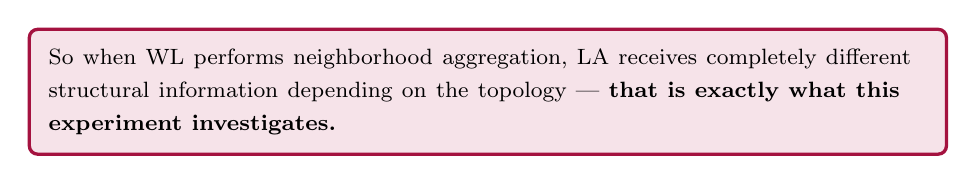
\begin{tikzpicture}
        \node[rectangle, draw=amritaMaroon, very thick, fill=maroonSoft,
              rounded corners=3pt, inner sep=7pt, text width=0.92\textwidth] {
            \footnotesize So when WL performs neighborhood aggregation, LA
            receives completely different structural information depending on
            the topology --- \textbf{that is exactly what this experiment
            investigates.}
        };
    \end{tikzpicture}
\end{frame}

% ============================================================
% FRAME: Where Are WL Graph Kernels Used? (Applications)
% ============================================================
\begin{frame}{Where Are WL Graph Kernels Used?}
    \framesubtitle{Applications of WL graph kernels}

    \footnotesize
    WL graph kernels are particularly useful when the input is naturally
    represented as graphs and the goal is to \textbf{classify or compare
    graph-structured data}.

    \vspace{0.4cm}
    \begin{columns}[T]
        \column{0.48\textwidth}
        \centering
        \iconGraph \\[4pt]
        \textbf{Graph Classification}\\[2pt]
        {\scriptsize\itshape Classify molecules, proteins, chemical
        compounds, etc.}

        \column{0.48\textwidth}
        \centering
        \iconMagnify \\[4pt]
        \textbf{Pattern Recognition}\\[2pt]
        {\scriptsize\itshape Identify structural patterns in graphs.}
    \end{columns}

    \vspace{0.55cm}
    \begin{columns}[T]
        \column{0.48\textwidth}
        \centering
        \iconDNA \\[4pt]
        \textbf{Bioinformatics}\\[2pt]
        {\scriptsize\itshape Compare molecular and biological structures.}

        \column{0.48\textwidth}
        \centering
        \iconLeaf \\[4pt]
        \textbf{Image / Plant Trait Analysis}\\[2pt]
        {\scriptsize\itshape Represent relationships among extracted
        features as graphs.}
    \end{columns}
\end{frame}

% ============================================================
% FRAME: Applications in the Literature (evidence slide)
% ============================================================
\begin{frame}{Applications in the Literature}
    \framesubtitle{WL graph kernels power real detection and comparison systems}

    \begin{center}
    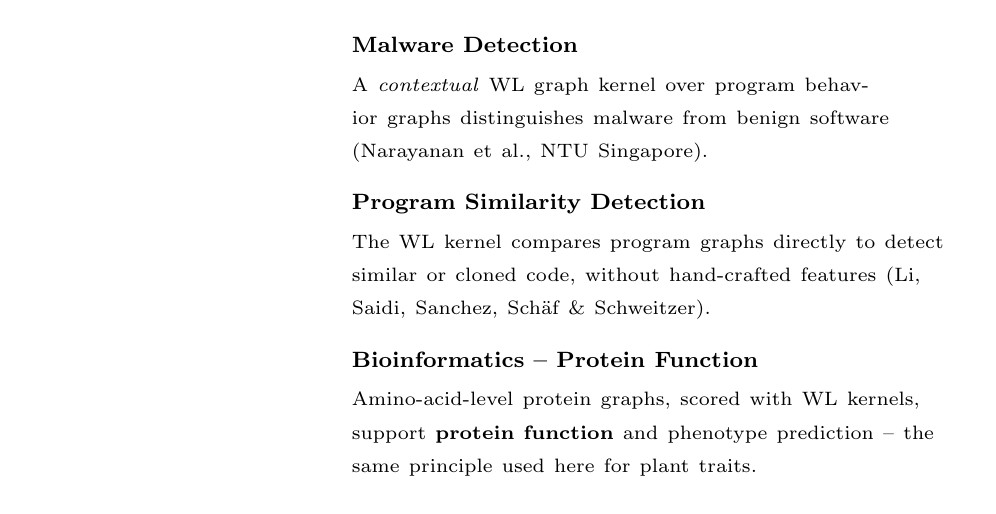
\begin{tikzpicture}[every node/.style={transform shape}]
        \node[anchor=north west, inner sep=0] (img1) at (0,0)
            {}; 
        \node[anchor=north west, text width=7.7cm, align=left] (txt1) at (4.0,0.05) {
            \footnotesize\textbf{Malware Detection}\\[2pt]
            \scriptsize A \emph{contextual} WL graph kernel over program
            behavior graphs distinguishes malware from benign software
            (Narayanan et al., NTU Singapore).
        };

        \node[anchor=north west, inner sep=0] (img2) at (0,-2.0)
            {};
        \node[anchor=north west, text width=7.7cm, align=left] (txt2) at (4.0,-1.95) {
            \footnotesize\textbf{Program Similarity Detection}\\[2pt]
            \scriptsize The WL kernel compares program graphs directly to
            detect similar or cloned code, without hand-crafted features
            (Li, Saidi, Sanchez, Sch\"af \& Schweitzer).
        };

        \node[anchor=north west, inner sep=0] (img3) at (0,-4.0)
            {};
        \node[anchor=north west, text width=7.7cm, align=left] (txt3) at (4.0,-3.95) {
            \footnotesize\textbf{Bioinformatics -- Protein Function}\\[2pt]
            \scriptsize Amino-acid-level protein graphs, scored with WL
            kernels, support \textbf{protein function} and phenotype
            prediction -- the same principle used here for plant traits.
        };
    \end{tikzpicture}
    \end{center}

    \vspace{0.05cm}
    {\scriptsize\itshape Across security, software engineering, and biology,
    the same idea recurs: represent structure as a graph, let WL capture
    its neighborhoods, and compare.}
\end{frame}

% ============================================================
% FRAME: How Does the WL Graph Kernel Perform Classification?
% ============================================================
\begin{frame}{How Does the WL Graph Kernel Perform Classification?}
    \framesubtitle{From plant graph to predicted class}

    \begin{center}
    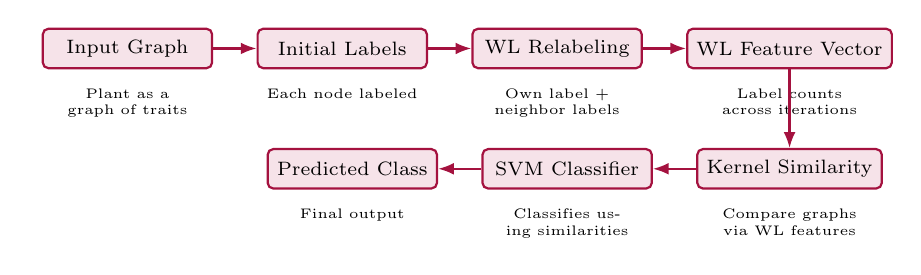
\begin{tikzpicture}[every node/.style={transform shape}]
        \tikzset{
            wlbox/.style={rectangle, draw=amritaMaroon, thick, fill=maroonSoft,
                rounded corners=2pt, minimum width=2.15cm, minimum height=0.5cm,
                font=\scriptsize, align=center},
            wlcap/.style={font=\tiny, align=center, text width=2.3cm}
        }
        % Row 1: left to right
        \node[wlbox] (b1) at (0,0) {Input Graph};
        \node[wlbox, right=0.55cm of b1] (b2) {Initial Labels};
        \node[wlbox, right=0.55cm of b2] (b3) {WL Relabeling};
        \node[wlbox, right=0.55cm of b3] (b4) {WL Feature Vector};

        \node[wlcap, below=0.12cm of b1] (c1) {Plant as a graph of traits};
        \node[wlcap, below=0.12cm of b2] (c2) {Each node labeled};
        \node[wlcap, below=0.12cm of b3] (c3) {Own label + neighbor labels};
        \node[wlcap, below=0.12cm of b4] (c4) {Label counts across iterations};

        % Row 2: right to left, continuing the flow
        \node[wlbox, below=1.0cm of b4] (b5) {Kernel Similarity};
        \node[wlbox, left=0.55cm of b5] (b6) {SVM Classifier};
        \node[wlbox, left=0.55cm of b6] (b7) {Predicted Class};

        \node[wlcap, below=0.12cm of b5] (c5) {Compare graphs via WL features};
        \node[wlcap, below=0.12cm of b6] (c6) {Classifies using similarities};
        \node[wlcap, below=0.12cm of b7] (c7) {Final output};

        \draw[-{Latex[length=2mm]}, thick, draw=amritaMaroon] (b1) -- (b2);
        \draw[-{Latex[length=2mm]}, thick, draw=amritaMaroon] (b2) -- (b3);
        \draw[-{Latex[length=2mm]}, thick, draw=amritaMaroon] (b3) -- (b4);
        \draw[-{Latex[length=2mm]}, thick, draw=amritaMaroon] (b4) -- (b5);
        \draw[-{Latex[length=2mm]}, thick, draw=amritaMaroon] (b5) -- (b6);
        \draw[-{Latex[length=2mm]}, thick, draw=amritaMaroon] (b6) -- (b7);
    \end{tikzpicture}
    \end{center}

    \vspace{0.1cm}
    \begin{center}
    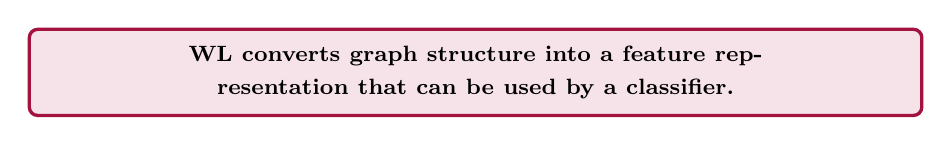
\begin{tikzpicture}
        \node[rectangle, draw=amritaMaroon, very thick, fill=maroonSoft,
              rounded corners=3pt, inner sep=6pt, text width=0.9\textwidth, align=center] {
            \footnotesize\textbf{WL converts graph structure into a feature
            representation that can be used by a classifier.}
        };
    \end{tikzpicture}
    \end{center}

    \vspace{0.12cm}
    \begin{center}
    {\scriptsize\itshape The topology determines which neighboring labels WL
    can see.}

    \vspace{0.1cm}
    {\footnotesize\bfseries Same traits + same WL kernel + different graph
    topology $\rightarrow$ different WL information $\rightarrow$ potentially
    different classification performance}
    \end{center}
\end{frame}

% ============================================================
% FRAME: Research Implementation Overview
% ============================================================
\begin{frame}{Research Implementation Overview}
    \framesubtitle{Experimental Pipeline for OLID Dataset}

    \begin{itemize}
        \item \textbf{Dataset:} Olive Leaf Image Dataset (OLID).
        \item \textbf{Feature Extraction:} Morphological, color, and texture features were extracted.
        \item \textbf{Graph Construction Models Evaluated:}
        \begin{itemize}
            \item \textbf{Star Graph Topology:} A central root node connected to all feature nodes.
            \item \textbf{Fully Connected Topology:} Every feature node connected to every other node.
            \item \textbf{Attribute-Aware Models:} Enriching the representation using continuous node features instead of purely discrete ones.
        \end{itemize}
        \item \textbf{Evaluation metric:} Support Vector Machine (SVM) Classification Accuracy comparing different WL graph structures.
    \end{itemize}
\end{frame}

% ============================================================
% FRAME: Key Findings & Evaluation
% ============================================================
\begin{frame}{Key Findings \& Evaluation}
    \framesubtitle{Comparing Topologies}

    \begin{columns}[c]
        \column{0.5\textwidth}
        \textbf{Topology Performance Variations}
        \vspace{0.15cm}
        \begin{itemize}
            \item \textbf{Star Graph:} Provides a strong baseline by capturing relationships between the central entity (Plant) and its traits.
            \item \textbf{Fully Connected Graph:} Captures the covariance and pairwise interactions between different leaf traits (e.g., how Leaf Area relates to Venation).
        \end{itemize}
        \column{0.5\textwidth}
        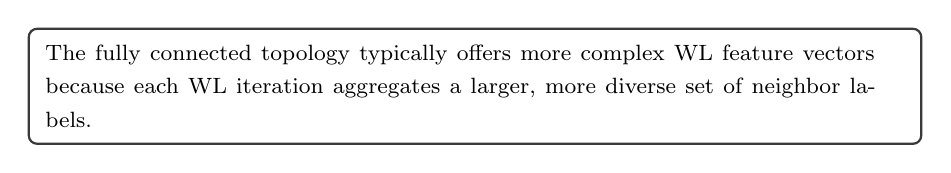
\begin{tikzpicture}
            \node[rectangle, draw=inkGray, thick, fill=white,
                  rounded corners=3pt, inner sep=6pt, text width=0.9\textwidth] {
                \footnotesize The fully connected topology typically offers more complex WL feature vectors because each WL iteration aggregates a larger, more diverse set of neighbor labels.
            };
        \end{tikzpicture}
    \end{columns}
\end{frame}

% ============================================================
% FRAME: Conclusion
% ============================================================
\begin{frame}{Conclusion}
    \begin{itemize}
        \item Graph topology significantly affects the discriminative power of Weisfeiler-Lehman kernels.
        \item While WL kernels are powerful, their success depends heavily on \textbf{how the graph is constructed} from tabular/image features.
        \item Continuous, Attribute-Aware Graph Kernels further refine classification by mitigating the information loss present in purely discrete label aggregation.
    \end{itemize}
    \vspace{0.5cm}
    \begin{center}
        \Large \textbf{Thank You!}
    \end{center}
\end{frame}

\end{document}
